\documentclass[12pt]{article}
\usepackage[utf8]{inputenc}
\usepackage[T1]{fontenc}
\usepackage{pdflscape} 
\usepackage{lmodern}
\usepackage{amsmath}
\usepackage[a4paper,bindingoffset=0.2in,%
            left=0.5in,right=0.5in,top=0.5in,bottom=1in,%
            footskip=.25in]{geometry}
\usepackage[colorlinks=true, linkcolor=Black, urlcolor=Blue]{hyperref}
\usepackage{graphicx}
\usepackage{subcaption}
\usepackage{listings}
\usepackage{color}
\usepackage{float}
\usepackage[usenames, dvipsnames]{xcolor}

\definecolor{codegreen}{rgb}{0,0.6,0}
\definecolor{codegray}{rgb}{0.5,0.5,0.5}
\definecolor{codepurple}{rgb}{0.58,0,0.82}
\definecolor{backcolour}{rgb}{0.95,0.95,0.92}

\lstdefinestyle{mystyle}{
	backgroundcolor=\color{backcolour},   
	commentstyle=\color{codegreen},
	keywordstyle=\color{magenta},
	numberstyle=\tiny\color{codegray},
	stringstyle=\color{codepurple},
	basicstyle=\ttfamily\footnotesize,
	breakatwhitespace=false,         
	breaklines=true,                 
	captionpos=b,                    
	keepspaces=true,                 
	numbers=left,                    
	numbersep=5pt,                  
	showspaces=false,                
	showstringspaces=false,
	showtabs=false,                  
	tabsize=2
}


\begin{document}
\title{Projekt 2: Analiza możliwości algorytmów optymalizacji\\
\large Sebastian Michoń 136770, Marcin Zatorski 136834\\
\large grupa L5}
\date{\vspace{-10ex}}
\maketitle

\section{Zarys idei}
\begin{enumerate}
	\item Obliczenia przeprowadzano dla 2 architekur:
	\begin{enumerate}
		\item Standardowa sieć neuronowa, złożona z warstw gęstych o kolejno 10-50-100-100-100-5 neuronach (10 neuronów wejściowych, 5 wyjściowych).
	\end{enumerate}
	\item Operacje przeporwadzone dla pierwszej architektury:
	\begin{enumerate}
		\item Stworzono pewną sieć neuronową i dane treningowe i testowe. Dane treningowe składały się z 50.000 instancji, dane testowe z 10.000 instancji.
		\item Uruchamiano losowo zainicjalizowaną (z biasem z rozkładu normalnego) sieć neuronową dla danych treningowych. Będzie ona nazywana dalej wzorcową siecią neuronową.
		\item W każdym pojedynczym eksperymencie porównywano określone optymalizatory w zdefiniowany sposób:
		\begin{enumerate}
			\item Ustalano ground truth jako rezultat propagacji zestawu treningowego i testowego przez sieć neuronową z wagami pochodzącymi z wzorcowej sieci neuronowej i regularyzacją (gdyby używać wzorcowej sieci neuronowej z takimi samymi wagami i bez regularyzacji, wyniki mogłyby się różnić dla regularyzacji 'batch  normalization'; Dzięki rozwiązaniu zadania w taki sposób spełniono założenie o identycznej architekturze sieci neuronowych jednocześnie - dzięki kopiowaniu wag - umożliwiając porównywanie rezultatów dla różnych rodzajów regularyzacji).
			\item Tworzono sieć neuronową dla podanej metody regularyzacji i podanego hiperparametru (np. dropout\_rate=0.2). Nazywana ona będzie dalej testową sięcią neuronową
			\item Trenowano testową sieć neuronową w 3 epokach.
			\item Po wytrenowaniu testowej sieci neuronowej ewaluowano ją na zbiorze treningowym, testowym i porównywano wagi w dwóch sieciach neuronowych: testowej i wzorcowej.
		\end{enumerate}
	\end{enumerate}
	\item Dla pierwszej architektury eksperymenty przeprowadano dla następujących typów normalizacji:
	\begin{enumerate}
		\item \textbf{batch\_normalization}: przeprowadzano testy dla 3 optymalizatorów: SGD, Adam i AdamW(weight\_decay = 0.0001). Przeprowadzono testy dla każdej pary wartości z ciągu [4, 16, 64, 256] dla parametru batch\_size i wartości z ciągu [0.1, 0.5, 0.9, 0.95, 0.99, 0.999] dla parametru momentum - w sumie wykonano 24 testy dla tej normalizacji.
		
		\item \textbf{weight\_decay}: przeprowadzano testy dla 2 optymalizatorów: SGDV i AdamW. Przeprowadzono testy dla każdej wartości z ciągu [0.5, 0.1, 0.01, 0.001, 0.0001, 0.00001] dla parametru weight\_decay - w sumie wykonano 6 testów dla tej normalizacji.
		
		\item \textbf{dropout}: przeprowadzano testy dla 3 optymalizatorów: SGD, Adam i AdamW(weight\_decay = 0.0001). Przeprowadzono testy dla każdej wartości z ciągu [0, 0.1, 0.2, 0.3, 0.4, 0.5] dla parametru dropout\_rate - w sumie wykonano 6 testów dla tej normalizacji.
	\end{enumerate}
	Wykonano zatem w sumie 36 testów. Wartwy Dropout / Batch normalization wstawiono pomiędzy każdą parę warstw gęstych z wyłączeniem pierwszych 2 warstw (czyli na przykład 10-50-Dropout-100-Dropout-100-Dropout-100-Dropout-5).
	
	
	\item \label{tit:cost} Funkcja kosztu wag:
	\begin{enumerate}
		\item Zaimplementowano standardową funkcję liczącą MSE będący uśrednioną sumą błędów kwadratowych dla wag i biasa (liczonego w średniej jako jedna z wag). \item Aby porównywać wagi neuronów, które są w jakiś sposób związane, przed wyliczeniem funkcji kosztu modyfikowano macierze wag w wytrenowanej testowej sieci neuronowej tak, aby neurony, które mają podobne wartości wag i biasa na wejściu były na tych samych pozycjach w obydwu porównywanych sieciach neuronowych.
		\item Dla wszystkich macierzy wag i biasów - począwszy od pierwszej - porównywano ujemne podobieństwo kosinusowe pomiędzy każdą parą wektorów wag (z biasem) dla pojedynczego neurona w obu sieciach. Wektor wag wchodzących do neurona był kolumną macierzy wag poprzedzającej daną warstwę (np. na samym początku - dla warstw o rozmiarach 10,50 - macierz wag miała rozmiar 10x50, zaś wektor wag wchodzących do pojedynczego neurona miał rozmiar 10x1, uwzględniając bias 11x1).
		\item Celem metody była maksymalizacja podobieństwa neuronów na tych samych pozycjach; w tym celu wykorzystano metodę węgierską, aby wybrać minimalną możliwą sumę ujemnych podobieństw kosinusowych przy pewnej zamianie miejscami pozycji neuronów. Rezultatem metody węgierskiej była sekwencja par $1:a_1, 2:a_2, \dots m:a_m$ oznaczająca, że aby zminimalizować sumę ujemnych podobieństw kosinusowych wektorów wag (z biasem) dla pojedynczego neurona należy dokonać takiej transformacji na macierzy wag, aby kolumna o indeksie $a_i$ była na pozycji \(i\)-tej po transformacji testowej sieci neuronowej. Transormację tę osiągnięto przez:
		$$\begin{bmatrix}
			k_1 & k_2 \dots k_m\\
		\end{bmatrix}
		\begin{bmatrix}
			e_{a_1} & e_{a_2} & \dots e_{a_m}\\
		\end{bmatrix}
		=
		\begin{bmatrix}
			k'_1 & k'_2 & \dots k'_m\\
		\end{bmatrix}
		$$
		gdzie \(e_i\) oznacza pionowy wektor jednostkowy o wypełniony zerami i jedną jedynką w pozycji \(i\)-tej, wektory jednostkowe mają rozmiar \(m\) (macierz z prawej jest kwadratowa), wektory \(k\) to kolumny macierzy wag przed transformacją. W ten sam sposób transformowano wektor biasów.
		\item Analogicznie, jeśli za daną warstwą była inna wartswa gęsta, zamienian kolejnością wiersze następnej macierzy wag tak, aby kolejność neuronów była taka sama w obu macierzach (a zatem należało zmienić kolejność wartości wychodzących z poprzedniej warstwy).
		$$\begin{bmatrix}
			e_{a_1}^T\\ e_{a_2}^T\\ \dots\\ e_{a_m}^T\\
		\end{bmatrix}
		\begin{bmatrix}
			w'_1\\ w'_2\\ \dots\\ w'_m\\
		\end{bmatrix}
		=
		\begin{bmatrix}
			w'_1\\ w'_2\\ \dots\\ w'_m\\
		\end{bmatrix}
		$$. Nie transformowano wektora biasów, ponieważ nie miał on związku z transformacją pozycji wyjść z poprzedniej warstwy.
	\end{enumerate}
\end{enumerate}
\section{Rezultaty i ich omówienie}
\subsection{Testy pierwszej sieci}
\subsubsection{Testy batch\_normalization}
\begin{figure}[h!]
	\centering
	\begin{subfigure}[b]{1\linewidth}
		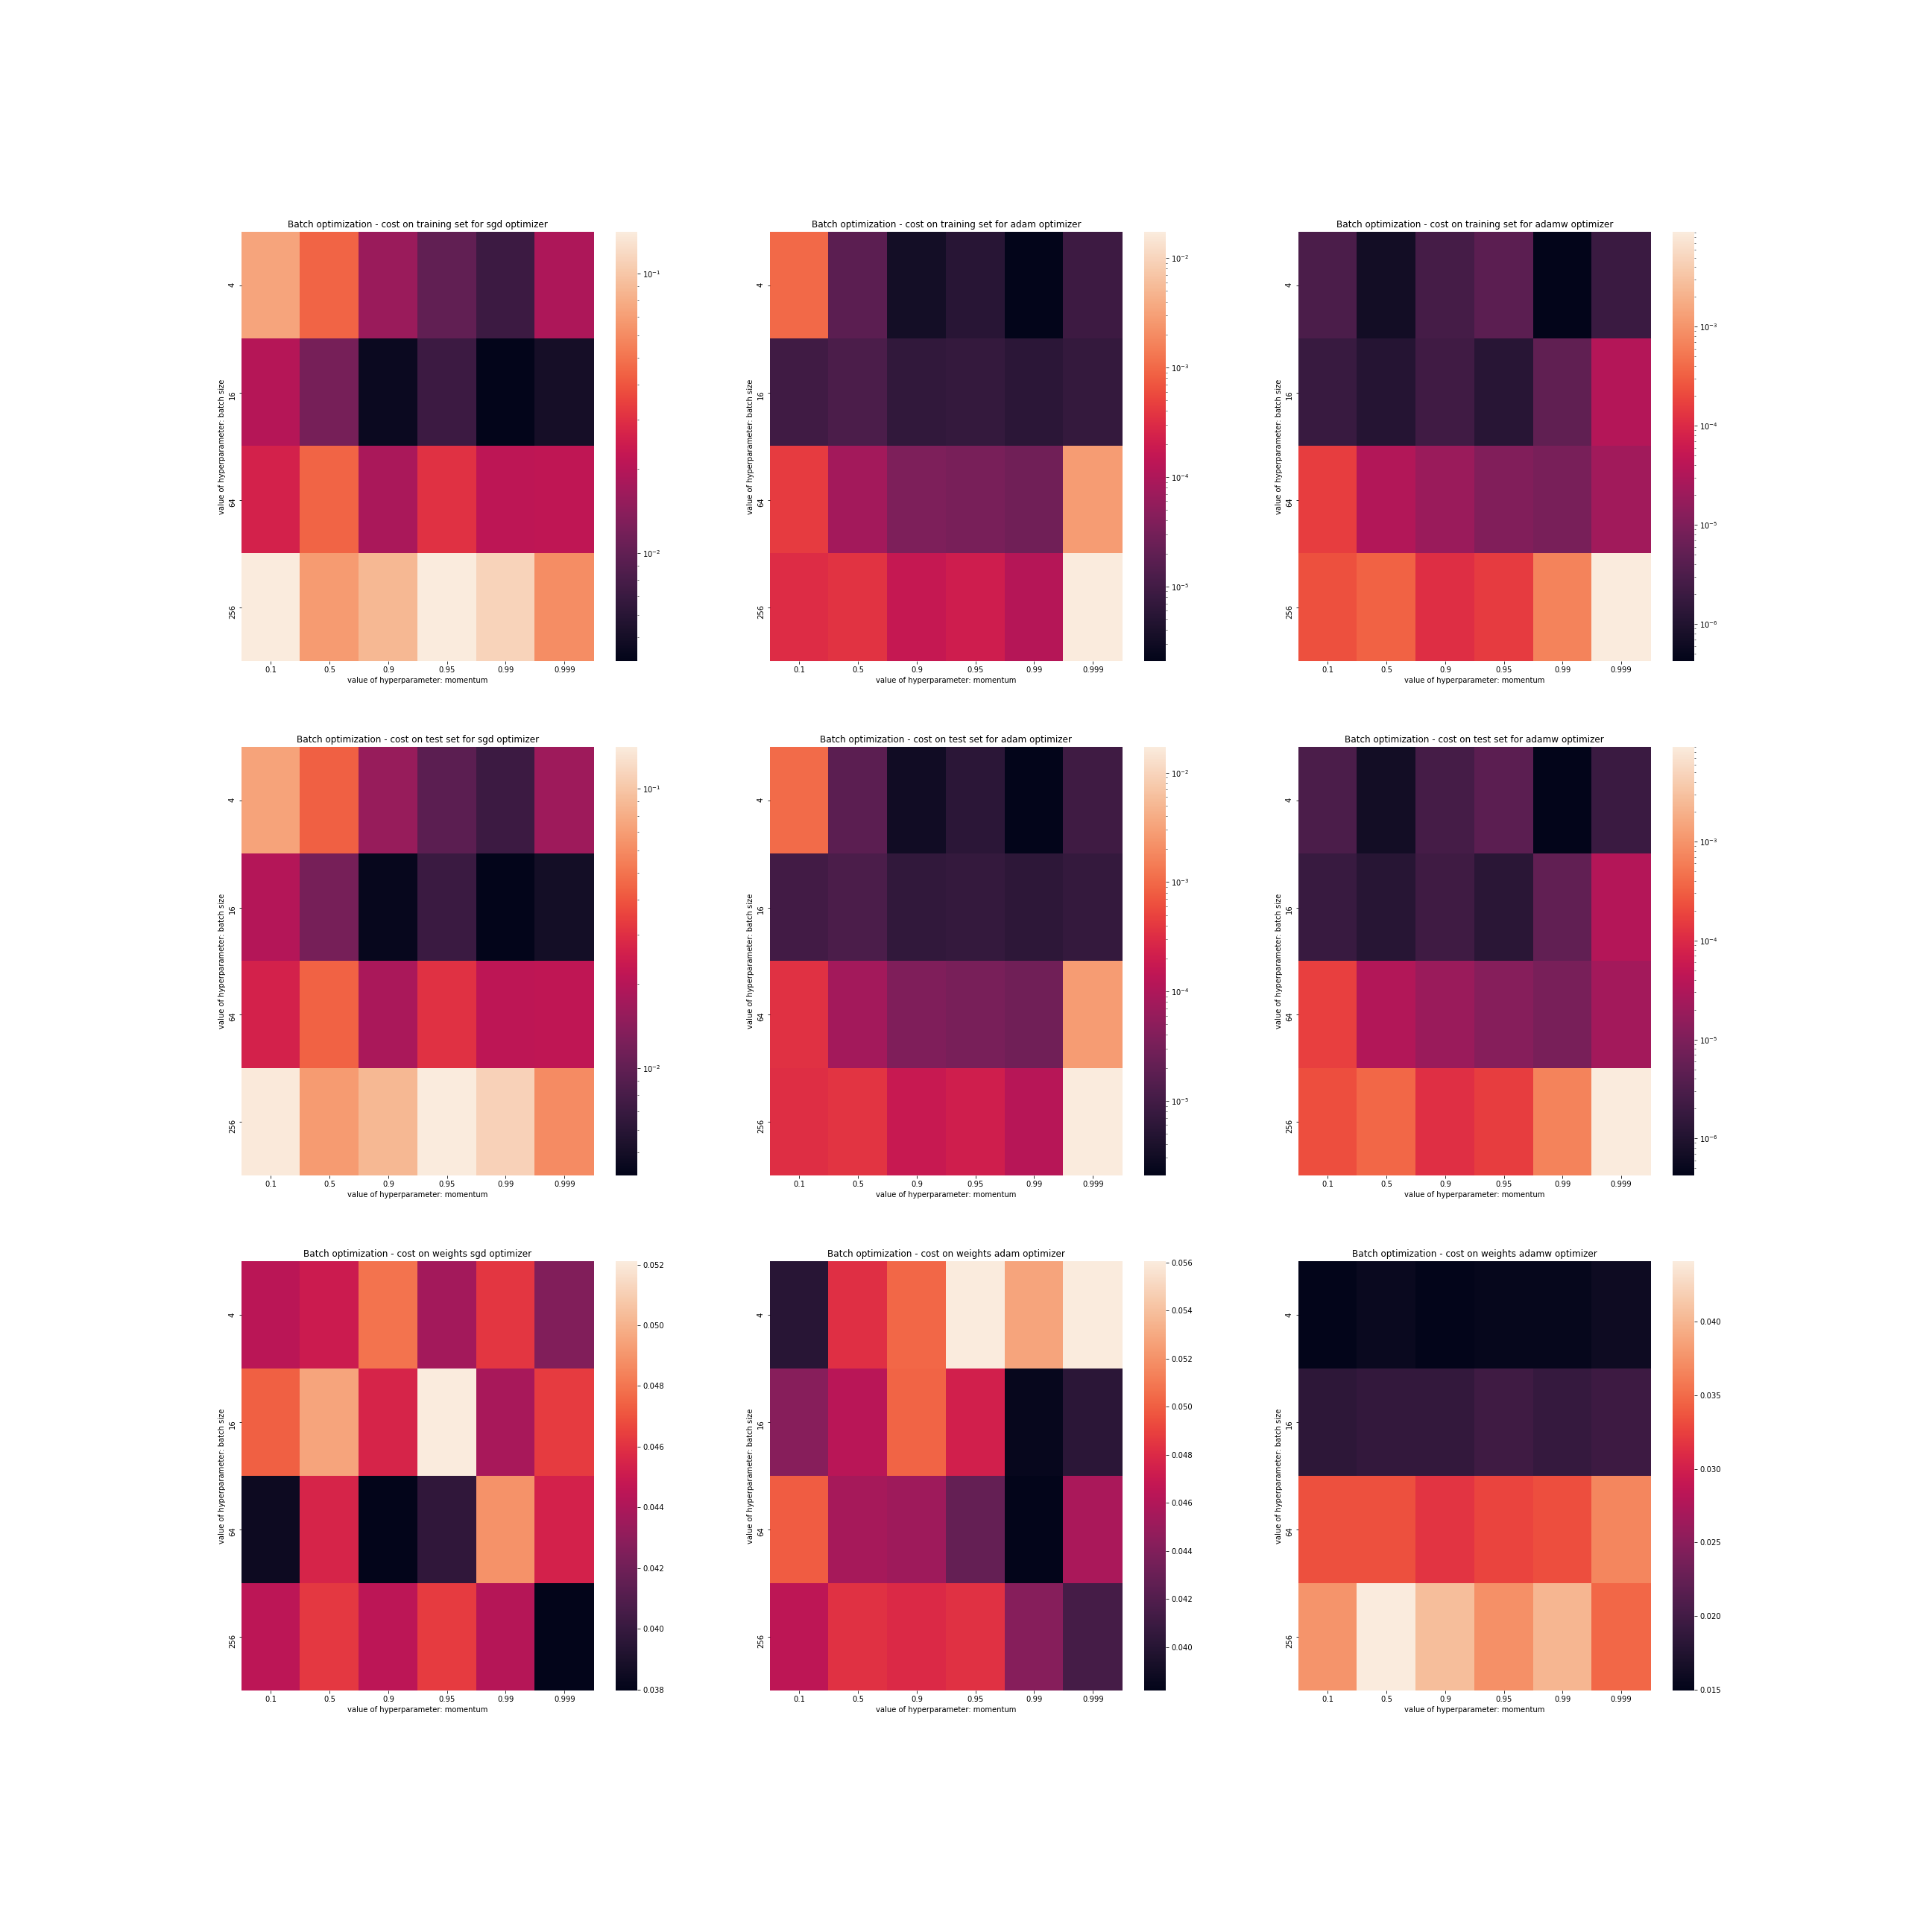
\includegraphics[width=\linewidth]{Comparision_batch_norm.png}
	\end{subfigure}
	\label{fig:batch}
	\caption{Rezultaty testowania rezultatów nauki sieci z normalizacją typu batch normalization}
\end{figure}
Opis testów i ich rezultatów:
\begin{enumerate}
	\item Na tym i każdym kolejnym wykresie wartości funkcji kosztu dla zestawu testowego i treningowego będą przedstawiane w skali logarytmicznej, nawet dla SGD.
	\item Wartości funckji kosztu dla zbioru treningowego i testowego są nieomal identyczne - wynika to z:
	\begin{enumerate}
		\item 50.000 Instancji danych treningowych pochodzących z tego samego rozkładu - pociąga to za sobą możliwość efektywnego wytrenowania sieci.
		\item Braku szumu w danych wyjściowych - Wzorcowe wartości na wyjściu są funkcją zależną jedynie od inputu.
		\item Identycznej struktury obu sieci neuronowych.
	\end{enumerate}
	Obserwacja ta będzie zauważalna we wszystkich kolejnych testach.
	\item Najlepsze rezultaty optymalizacji SGD (wartość MSE rzędu około 0.01) są porównywalne z najgorszymi rezultatami optymalizacji Adam i AdamW. Obserwacja ta będzie się powtarzała w kolejnych testach.
	\item Wszystkie optymalizatory uzyskały najniższe wartości funkcji kosztu dla momentum=0.99.
	\item Dla SGD najlepsze wyniki osiągano dla batch\_size=16, dla Adam i AdamW dla batch\_size=4.
	\item Wartości fukcji kosztu dla batch\_size wyższego równego 64 są prawie zawsze wyższe niż dla mniejszego batch\_size.
	\item AdamW dla batch\_size=4 bardzo dobrze dopasowywał się do wag sieci wzorcowej; żaden inny optymalizator nie osiągnął podobnych rezultatów dla opisanej w paragrafie \ref{tit:cost} funckji kosztu (0.15 AdamW względem 0.38 SGD i Adama). W ogólności Adam\_W lepiej dopasowywał wagi do sieci wzorcowej niż pozostałe optymalizatory.
	\item Dla wartości funckji kosztu osiąganej przez optymalizaotry Adam i AdamW niemożliwość perfekcyjnego dopasowania do wzorcowej sieci neuronowej może wynikać między innymi z błędów zaokrągleń.
\end{enumerate}

\subsubsection{Testy weight\_decay}
\begin{figure}[H]
	\centering
	\begin{subfigure}[b]{1\linewidth}
		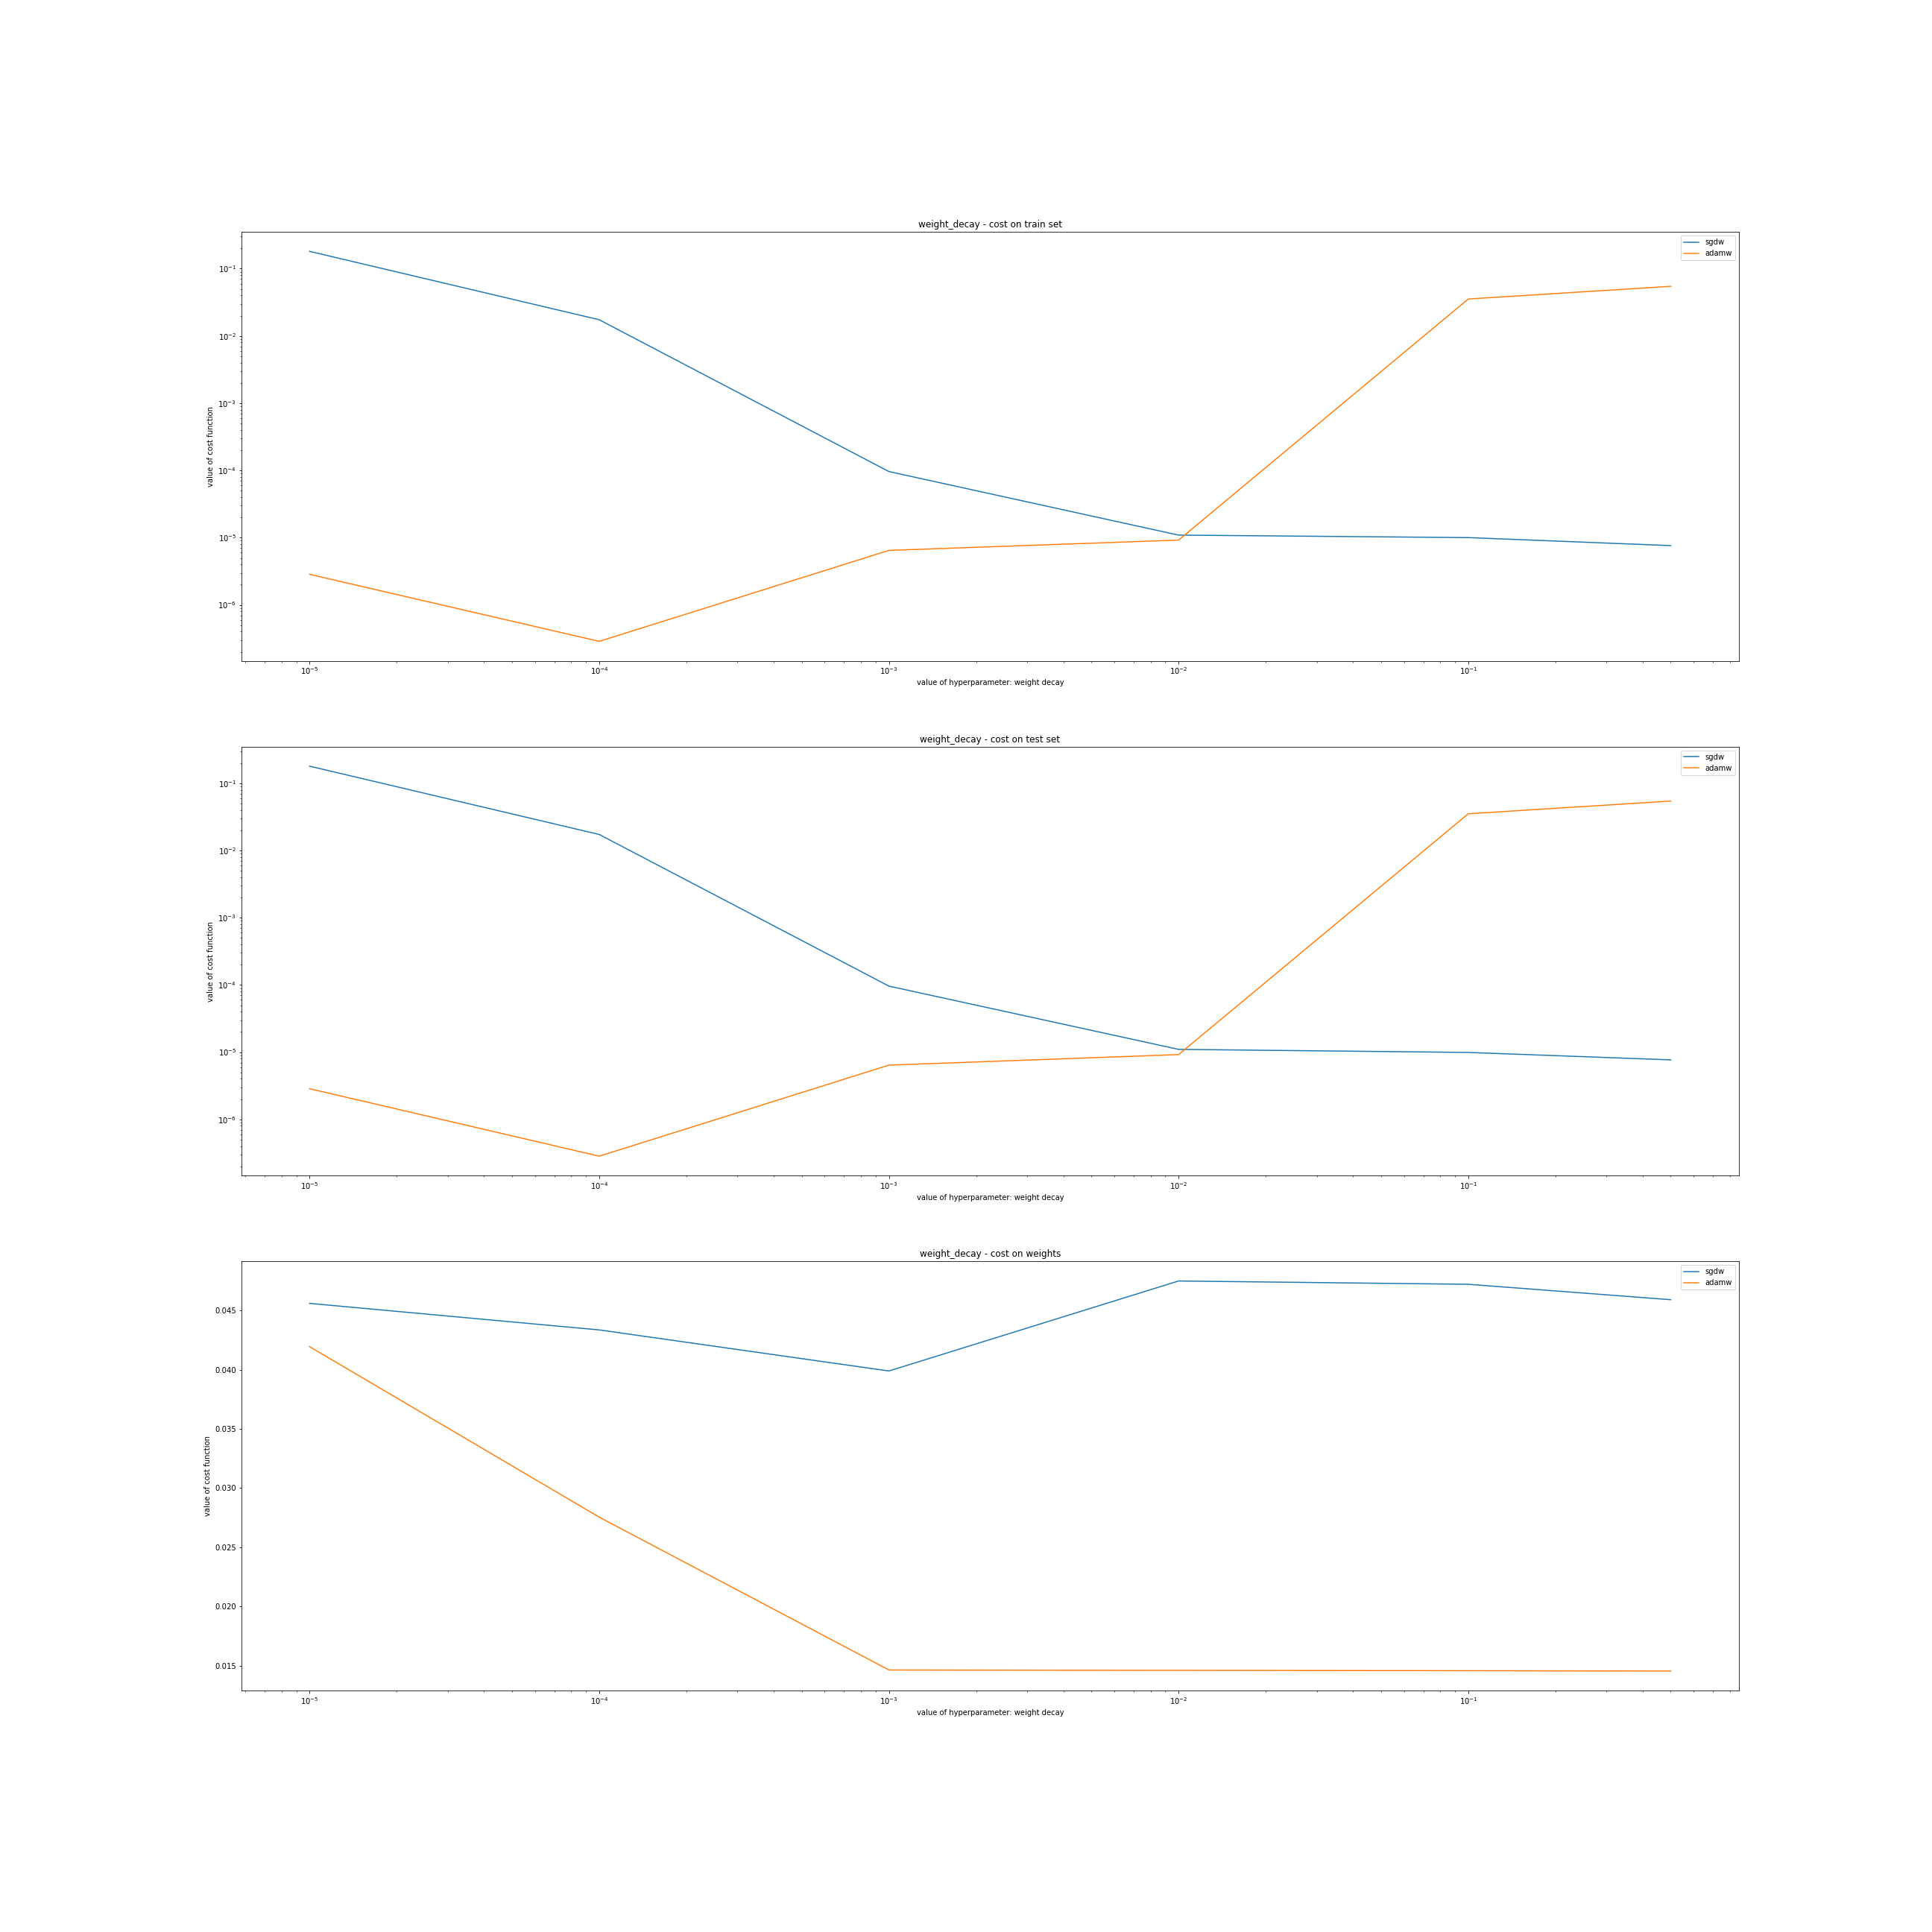
\includegraphics[width=\linewidth]{Comparision_weight_decay.png}
	\end{subfigure}
	\label{fig:decay}
	\caption{Rezultaty testowania rezultatów nauki sieci z róznymi wartościami weight decay w optymalizatorze.}
\end{figure}
Opis testów i ich rezultatów:
\begin{enumerate}
	\item Skale na obu osiach są skalami logarytmicznymi z wyjątkiem ostatniego rysunku, gdzie na osi y jest skala liniowa.
	\item Optymalizator SGDW osiągał najlepsze rezlutaty dla weight decay większego niż 0.1, z kolei AdamW osiągał najlepsze rezultaty dla weight decay rzędu \(10^{-4}\).
	\item Pomimo ponad stukrotnie wyższej wartości funkcji kosztu dla zestawu testowego i treningowego dla AdamW niż SGDW dla weight decay rzędu 0.1, funkcja kosztu dla wag była około 3 razy niższa dla algorytmu AdamW niż dla SGDW. W ogólności, funkcja kosztu wag była prawie stała dla SGDW (na poziomie 0.45) i malejąca dla AdamW.
	\item Najlepsze rezultaty osiągane przez SGDW i AdamW są podobne (około 10 razy niższe dla AdamW), co pokazuje wyższą skuteczność optymlizatora SGDW niż standardowego optymalizatora SGD.
\end{enumerate}

\subsubsection{Testy dropoutu}
\begin{figure}[H]
	\centering
	\begin{subfigure}[b]{1\linewidth}
		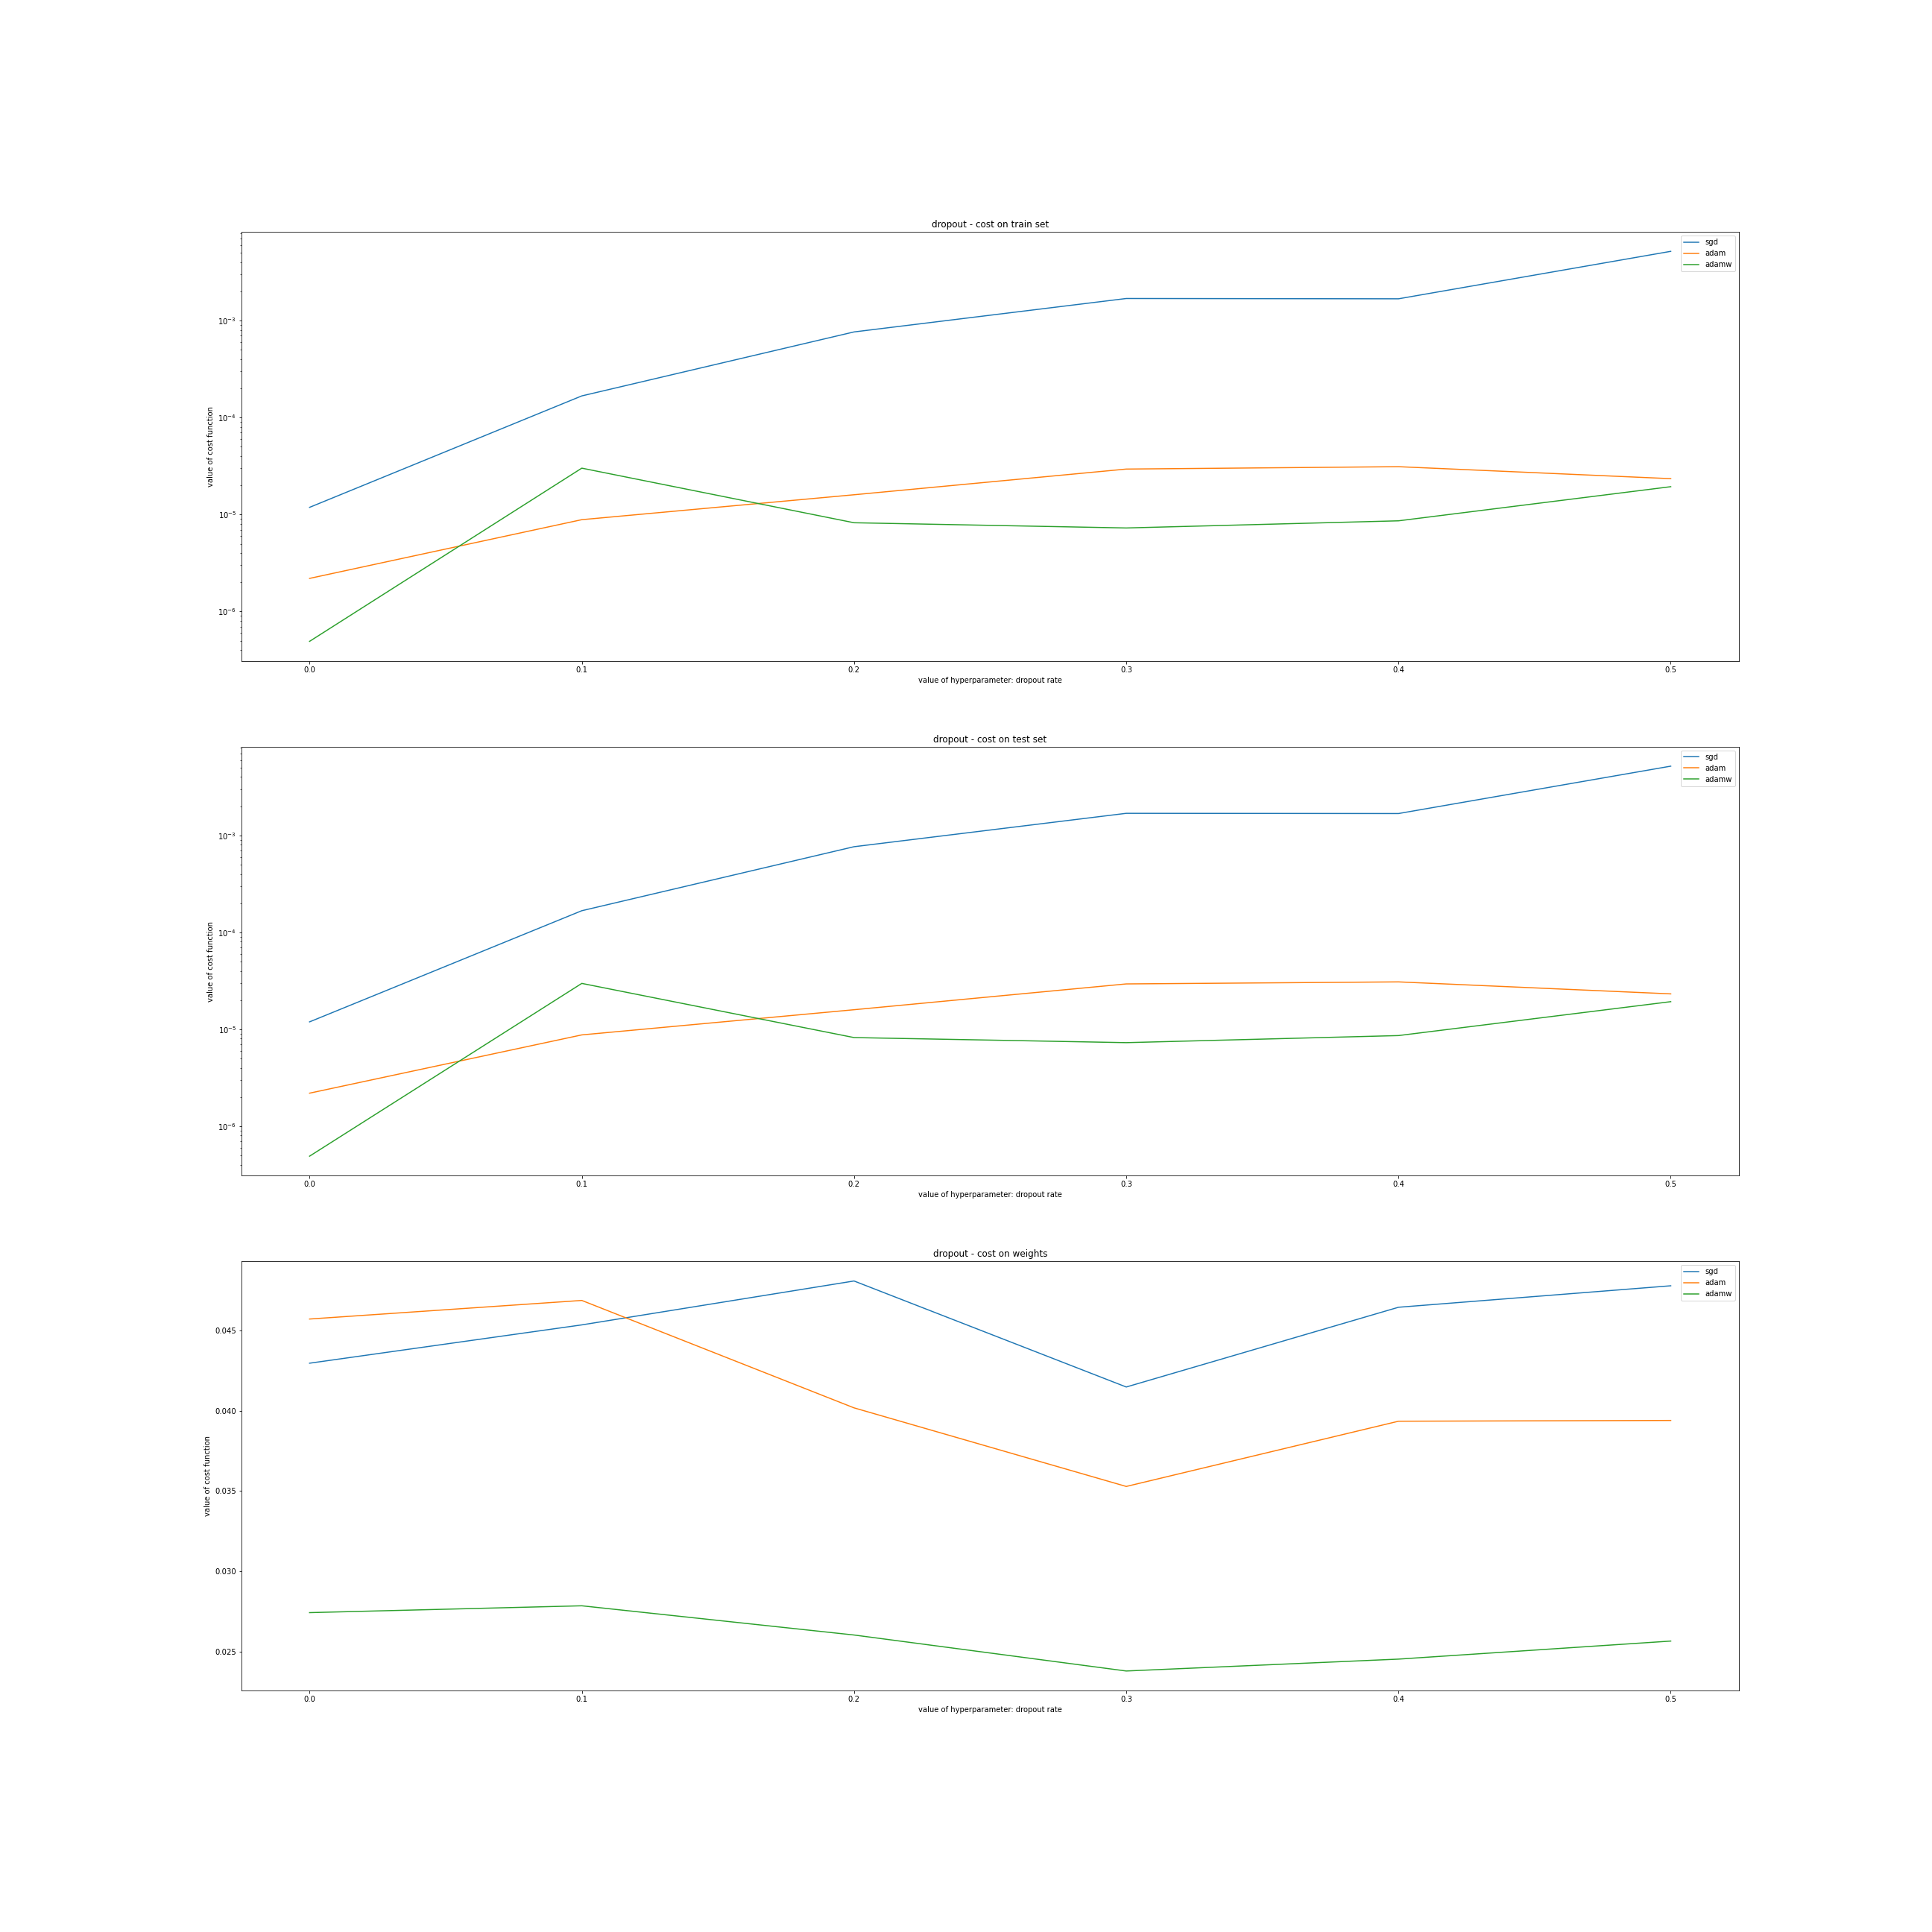
\includegraphics[width=\linewidth]{Comparision_dropout.png}
	\end{subfigure}
	\label{fig:decay}
	\caption{Rezultaty testowania rezultatów nauki sieci z róznymi wartościami weight decay w optymalizatorze.}
\end{figure}
Opis testów i ich rezultatów:
\begin{enumerate}
	\item Skale na osi y są skalami logarytmicznymi z wyjątkiem ostatniego rysunku, gdzie na osi y jest skala liniowa.
	\item Wzrost dropout rate często prowadził do wyższych wartości funkcji kosztu na zestawach treningowym i testowym - może to wynikać z kilku czynników:
	\begin{enumerate}
		\item Celem dodania dropoutu jest uniknięcie przetrenowania i dostosowania się sieci neuronowej do wyników obarczonym pewnym szumem; w tych danych nie ma żadnego szumu, teoretycznie można osiągnąć funkcję kosztu równą 0 dla każdych danych.
		\item Istnienie dropoutu może penalizować próbę upodobnienia sieci testowej do wzorcowej sieci neuronowej, np. przez odrzucanie neuronów istniejących we wzorcowej sieci mających kluczowy wpływ na rezultat.
	\end{enumerate}
	\item Optymalizator AdamW osiągał lepsze wyniki na obu zbiorach ze wzrostem dropoutu i dopasowywał się lepiej do wzorcowej sieci neurowej, osiągając minimum obu tych funkcji kosztu dla dropout\_rate=0.3.
	\item Wszystkie 3 optymalizatory osiągały najbardziej podobną sieć neuronową do sieci wzrocowej dla dropout\_rate=0.3.
	
\end{enumerate}

\clearpage

\section{Wnioski}
\begin{enumerate}
	\item Optymalizator SGD zawsze osiągał gorsze rezultaty niż AdamW z weight\_decay=$10^{-4}$, ponadto nie wykonywał się szybciej niż AdamW.
	\item Wykorzystanie optymalizatora AdamW z dobrze dopasowanym weight\_decay praktycznie zawsze prowadzi do lepszych rezultatów niż wykorzystanie optymalizatora Adam - zarówno w kontekście podobieństwa wag sieci neuronowych, jak i funkcji kosztu.
	\item Wartość weight\_decay ma bardzo duży wpływ na działanie optymalizatora, może powodować nawet osiągnięcie nawet $10^5$ razy mniejszej funkcji kosztu niż dowolna wartość tego hiperparametru. Optymalna wartość tego hiperparametru jest zależna od algorytmu.
\end{enumerate}

\end{document}
